\section{Specific effective constitutive model form for heart valve tissues replacements} \label{sec:specificform}

%%%%%%%%%%%%%%%%%%%%%%%%%%%%%%%%%%%%%%%%%%%%%%%%%%%%%%%%%%%%
%-------------------	begin FIGURE 	-------------------%
\begin{figure}
\centering
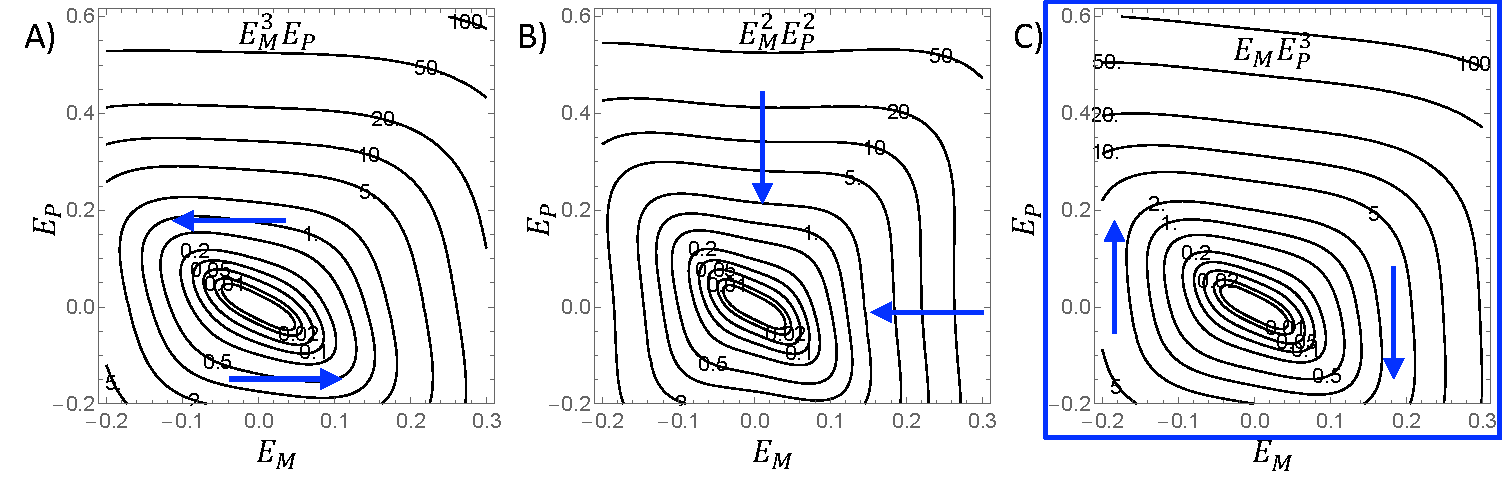
\includegraphics[width=6.5in]{Figures/couplingeffects}
\caption{The effect of the quartic coupling terms on the strain energy of $\Psi_{eff}$ (Eqn. \ref{eqn:finalexponentialmodelformscaled}). A) $E_m^3E_n$, shear of the $n$-axis. B)$E_m^2E_n^2$, squeezing. C)$E_mE_n^3$, shear of the $m$-axis.}
\label{fig:couplingeffects}
\end{figure}
%-------------------	 end FIGURE 	-------------------%
%%%%%%%%%%%%%%%%%%%%%%%%%%%%%%%%%%%%%%%%%%%%%%%%%%%%%%%%%%%%

    
	In some cases, it is possible to further reduce the form of $\Psi_{eff}$ (Eqn. \ref{eqn:finalexponentialmodelformscaled}). This may be helpful for reducing the cost of parameter estimation and parameter covariance. This depends on the coupling in the mechanical response of the material. For example, the $E_m$-$E_n$ coupling in most collagenous soft tissues (Fig. \ref{fig:couplingeffects}A) best match the behavior of the $E_m E_n^3$ term. This is because more fibers in the soft tissues are aligned to the material axis by definition, thus the effect of fiber rotation and thus coupling along this axis is generally less significant. Since $E_m^3 E_n$, $E_m^2 E_n^2$, and $E_m E_n^3$ are highly covariant terms in $\Psi{eff}$ (Eqn. \ref{eqn:finalexponentialmodelformscaled}). Each term affects the response of $\Psi_{eff}$ differently. Namely $E_m^2 E_n^2$ increases or decreases the roundedness of the contours (Fig. \ref{fig:couplingeffects}B), $E_m^3 E_n$ causes a shear of the S-axis (Fig. \ref{fig:couplingeffects}A), and $E_m E_n^3$ causes the shear of the M-axis (Fig. \ref{fig:couplingeffects}C). However, there is a only modest difference between the quality of fit between any combination of these three terms, $\Delta R^2<0.01$. Of these $E_m E_n^3$ gives the lowest $R^2$ and thus only $E_m E_n^3$ is necessary for $\Psi_{eff}$. Likewise, $E_m E_n E_\phi^2$ may not be needed due to low coupling between $E_m$-$E_n$, as observed in Sun et al. \cite{sun_biaxial_2003}. In some cases, it may be beneficial to separate the response of the matrix from those of collagen fiber and other components of the tissue, so it can be updated independently by the micro-models. In this case, $E_\phi^2$ is not necessary as the matrix modulus, thus the shear modulus, is zero and the $E_\phi^4$ will be able to describe shear stresses due to collagen fibers. As such, an example of the reduce form of the effective constitutive model for heart valve tissue replacements is
%==========================================================%
%-------------------	begin EQUATION 	-------------------%
\begin{equation}
\begin{aligned}\label{eqn:finalmodelform}
\Psi	=& c_0 \left(e^{Q} - 1\right) + \frac{\eta_M}{2} \left( \frac{1}{a}\left( I_1 -3\right)^{a} + \frac{r}{b} \left( I_1 -3\right)^{b} \right) - p\left(\mathrm{J}-1\right)\\
Q		=& b_1 E_m^2 + b_2 E_n^2 + b_4 E_m E_n + b_5 E_m^4 + b_6 E_n^4 + b_9 E_m E_n^3	\\
	&+ b_{10} E_\phi^4 + b_{11} E_m^2E_\phi^2 + b_{12} E_n^2 E_\phi^2,
\end{aligned}
\end{equation}
%-------------------	 end EQUATION 	-------------------%
%==========================================================%
where $\alpha$, $\beta$, and $r$ are pre-specified constants, p is the Lagrange multiplier for incompressibility, $\mu_M$ is the matrix modulus, and $c_0, b_1,...b_{12}$ are the remaining model parameters.



